\documentclass[a4paper,12pt,twoside]{hmcpset}
\usepackage[utf8]{inputenc}
\usepackage[english]{babel}
\usepackage{fancyhdr}
\usepackage[margin=1in]{geometry}
\usepackage{graphicx}
\usepackage{amsmath}
\usepackage{mathtools}
\usepackage[mathscr]{euscript}
%\newcommand*{\ms}[1]{\ensuremath{\mathscr{#1}}}
\usepackage{lmodern} % math, rm, ss, tt
\usepackage[T1]{fontenc} 
\usepackage{tikz}
\usepackage{caption}

\pagestyle{fancy}
\fancyhf{}
\rhead{Spring 2019}
\chead{Section 5}
\lhead{\vspace{5mm} Math 147 Topology}
\rfoot{Page \thepage}
\linespread{1.3}

\renewcommand{\headrulewidth}{2pt}
\renewcommand{\footrulewidth}{2pt}

\graphicspath{ {./figures_theorems_sect_5/} } 

% info for header block in upper right hand corner
\begin{document}
\section*{5.1 Hausdorff, Regular and Normal Spaces.}

In the definition of a $T_1$ space, isn't it sufficient to simply
state that there exists an open set $U$ about $x$ such that $y \notin
U$? \\
\\

\begin{problem}[Theorem 5.1] A space $(X, \mathscr{T})$ is $T_1$ if
    and only if every point of $X$ is closed.
\end{problem}

\begin{proof}
    First we'll prove the forward direction.
    Suppose every point $x
    \in X$ is a closed set. Then $X - \{x\}$ is open, so 
    foe $y \in
    X$, $y \ne x$, 
    there exists an open set $U$ such that $y \in U$ and $U \cap
    \{x\} = \emptyset \implies x \notin U$. 
    Analogously, $X - \{y\}$ is open so 
    there exists
    an open set $V$ containing $x$ such that $x \in V$ but $y \notin
    V$. Since $x,y$ were arbitrary distinct points of $X$, we have
    that $X$ is a $T_1$ space. \\
    \\
    Now suppose that $X$ is a $T_1$ space. Consider an $x \in X$ and
    suppose for a contradiction 
    that $y \in X$, $y \ne x$ is a limit point of $\{x\}$. 
    Then every open set of $y$ must contain $x$. However, 
    this is not possible since $x$ and $y$ are distinct points, $X$ is
    $T_1$, and
    therefore there exists an open set $U$ containing $x$ such that $y
    \notin U$. Thus $y$ can't be a limit point, which means that no
    element in $X - \{x\}$ is a limit point of $\{x\}$. Therefore, $x$
    must be a closed set, and since $x$ was arbitrary this shows that
    every point of $X$ must be a closed set.
\end{proof}

\begin{exercise}[Exercise 5.2]
    Let $X$ be a space with the finite complement
    topology. Show that $X$ is $T_1$.
\end{exercise} 

\begin{solution}
    Observe that $X - \{x\}$ is an open set in the finite complement
    topology for all $x \in X$. Then its
    complement, $X - (X - \{x\}) = \{x\}$ is closed. Therefore 
    every point is a
    closed set, and by the Theorem 5.1 we have that $X$ is a $T_1$
    space.
\end{solution}

\begin{exercise}[Exercise 5.3]
    Show that $\mathbb{R}_{\text{std}}$ is
Hausdorff. 
\end{exercise}

\begin{solution}
Consider any two distinct points $x$ and $y$ in $\mathbb{R}$. Then
observe that we can construct the open sets $B(x, \epsilon/2)$ and
$B(y, \epsilon/2)$ where $|x - y| < \epsilon$ so that $B(x, \epsilon/2)$
and $B(y, \epsilon/2)$ are disjoint but $x \in B(x, \epsilon/2)$ and
$y \in B(y, \epsilon/2)$. Since $x, y$ were distinct and arbitrary,
we have that
$\mathbb{R}_{\text{std}}$ is a Hausdorff space.
\end{solution}

\begin{exercise}[Exercise 5.4]
    Show that $\mathbb{H}_{\text{bub}}$ is regular.
\end{exercise}

\begin{solution}
    We found earlier that all subsets of the $x$-axis are closed in
$\mathbb{H}_{\text{bb}}$. Thus if we have a closed subset $A$ and a
point $x \notin U$, we can use exercise 4.10(4) to show that there
must exist disjoint open sets $U$ and $V$ such that $x \in U$ and $A
\subset V$. Therefore, $\mathbb{H}_{\text{bub}}$ is regular.
\end{solution}

\begin{exercise}[Exercise 5.5]
    Show that $\mathbb{R}_{LL}$ is normal. 
\end{exercise}

\begin{solution}
Let $A$, $B$ be two disjoint closed sets. Consider $a \in A$, and observe
that $\mathbb{R}_{\text{LL}} - B$ is an open set containing $a$. Therefore, 
there exists a basis element $[x, y)$ such that $a \in [x, y) \subset 
\mathbb{R}_{\text{LL}} - B$. Therefore, 
$[a, y) \subset [x, y) \subset (\mathbb{R}_{\text{LL}} - B)$. Observe that 
we can create open sets $[a, y)$ for all $a \in A$. Thus let 
$U = \bigcup\limits_{a \in A} [a, y)$, which is open as it is the arbitrary 
union of open sets. Similarly, if we take a $b \in B$ and find a basic open 
set $[x', y')$ such that $b \in [x', y') \subset \mathbb{R}_{\text{LL}} -
A$, then we can define an open set $V = \bigcup\limits_{b \in B}[b, y')$.
\\
\\
Now $U$ and $V$ cannot intersect. Each member $[a, y')$ in the union 
of $U$ is a subset of $\mathbb{R}_{\text{LL}} - B$, while each member 
$[b, y')$ in the union of $V$ is a subset of $\mathbb{R}_{\text{LL}} - A$, 
and if they did intersect then this would require that for some $a \in A$, 
$b \in B$, $[a, y) \cap [b, y') \ne \emptyset$. However, this is impossible
as this would imply that either $b \in [a, y)$ or $a \in [b, y')$, which 
cannot happen since $[a, y) \subset \mathbb{R}_{\text{LL}} - B$ and 
$[b, y') \subset \mathbb{R}_{\text{LL}} - A$. Thus we have that $U \cap V =
\emptyset$. Since $A$ and $B$ were arbitrary disjoint closed sets in
$\mathbb{R}_{\text{LL}}$, we see that $X$ must be normal 
by the definition of normality.
\end{solution}

\begin{exercise}[Exercise 5.6]
    1. Consider $\mathbb{R}^2$ with the standard topology. Let $p \in
\mathbb{R}^2$ be a point not in a closed set $A$. Show that 
$$
\inf\{d(a, p) | a \in A\} > 0.
$$
(Recall that inf $E$ is the greatest lower bound of a set of real
numbers $E$.)\\
2. Show that $\mathbb{R}^2$ with the standard topology is regular. \\
3. Find two disjoint closed subsets $A$ and $B$ of $\mathbb{R}^2$ with
the standard topology such that 
$$
\inf\{d(a, b) | a \in A \text{ and } b \in B\} = 0
$$
4. Show that $\mathbb{R}^2$ with the standard topology is normal.
\end{exercise}

\begin{solution}
    \begin{enumerate}
        \item Firstly we know that $\inf\{d(a, p) | a \in A\} \ge 0$ since the
        distance function is always greater than or equal to zero. Thus we
        must simply show that it is not zero for any $a \in A$ where $p \notin
        A$. First, observe that since $p$ is not a limit point of $A$, there
        exists an open set $B(p, \epsilon)$ containing $p$ such that $B(p,
        \epsilon) \cap A = \emptyset$. Therefore, we have that $\inf\{d(a, p)
        | a \in A\} > \epsilon > 0$, proving the desired result. 
    
        \item Let $x \in \mathbb{R}^2$ and suppose $A$ is a closed set not
        containing $x$. Since $x$ is not a limit point in $A$, there exists an
        open set $U$ containing $x$ such that $U \cap A = \emptyset$. Thus let
        $B(x, \epsilon) \subset U$. Then if we take each point in $a \in A$
        and construct an open ball $B(a, \epsilon/2)$ where $\epsilon =
        \inf\{d(a, p) | a \in A\}$, then none of these balls intersect $U$. If
        we union these set of balls, we'll obtain an open set which contains
        $A$ but is disjoint with $x$. Thus by definition, $\mathbb{R}^2$ with
        the standard topology is regular. 
        
        \item Consider the set of points which lies on the line $x = 0$ and $y =
        \frac{1}{x}$. The function $y$ converges to the $y$-axis, and while
        these two are sets are closed and disjoint we see that the inf of
        their distances between their points converges to 0.
        
        \item     If we have two disjoint closed sets $A$ and $B$, then no point of
        one set is a limit point of the other. Construct a ball about each
        point of $a$ given by $B(a, r_a)$ where $r_a =
        \frac{1}{4}\inf\{d(a, b) | b \in B\}$. By part (a), we know that
        $r_a > 0$. Similarly, let us constuct balls about each point $b
        \in B$ of radius $r_b = \frac{1}{4}\inf\{d(a, b) | a \in A\}$
        given by $B(b, r_b)$ Now observe that no ball from the set $\{B(a,
        r_a)| a \in A\}$ intersects with any ball from the set $\{B(b,
        r_b)| b \in B\}$, and that $A \subset \bigcup\limits_{a \in A}B(a,
        r_a)$ and $B \subset \bigcup\limits_{b \in B}B(b, r _b)$. Since
        $A$ and $B$ were arbitrary closed sets, we must have that
        $\mathbb{R}^2$ is normal.
    \end{enumerate}
\end{solution}
Note: this can be done for all metric spaces, since we didn't
necessarily appeal to explicit properties of $\mathbb{R}^2$!


\begin{problem}[Theorem 5.7] 1. A $T_2$-space (Hausdorff) is a
$T_1$-space.\\
2. A $T_3$-space (regular and $T_1$) is a Hausdorff space, that is a
$T_2$-space.\\
3. A $T_4$-space (normal and $T_1$) is regular and $T_1$, that is, a
$T_3$-space.
\end{problem}

\begin{proof}
    \begin{enumerate}
        \item In a $T_2$-space, we have that for every $x$ distinct from $y$
        of the topological space, there are disjoint open sets $U, V$ such
        that $x \in U$ and $y \in V$. As an obvious consequence,
        for each $x \ne y$, there exists open sets $U, V$ such that 
        $x \in U$, $y \notin U$ and $y \in V$, $x \notin V$.
        Since this holds for all distinct $x, y \in X$, we can
        conclude that by defintion $X$ is also a $T_1$ space.

        \item Let $x, y$ be distinct. Since the space
        is 
        regular, and because $\{x\}$ is a closed set (by $T_1$), we know that for
        every $y$ distinct form $x$, there must exist disjoint open sets
        $U, V$ such that $\{x\} \subset U$ and $y \in V$. In other
        words, there exists disjoint open sets such that $x \in U$, $y
        \in V$. Thus by
        definition, we have a $T_2$ space.

        \item Observe that since we have a $T_1$, every point is a
        closed set.
        Furthermore, since we have normality, disjoint closed sets may be
        contained in disjoint open sets. Thus consider a closed set $A$
        and a point $x \notin A.$ Then since $\{x\}$ and $A$ are disjoint
        closed sets, we may construct disjoint open sets $U$, $V$ such
        that $\{x\} \subset U$ and $A \subset V$. By definition, this
        shows that $X$ is also a regular space. Since the space is
        regular, and $T_1$ by hypothesis, we know that the space must
        be $T_3$ as desired.
    
        
    \end{enumerate}

\end{proof}

\begin{problem}[Theorem 5.8] A topological space $X$ is regular if and
    only if for each point $p$ in $X$ and open set $U$ containing $p$
    there exists an open set $V$ such that $p \in V$ and $\overline{V}
    \subset U$.
\end{problem}

\begin{proof}
    First we prove the forward direction.
    Suppose that $X$ is regular and consider some $p \in X$. \\
    Then let $p \in U \subset X$ where $U$ is an open set in $X$. Observe
    that $U^c$ is closed and $p \notin U^c$. By regularity, there must
    exist disjoint open sets $V, W$ such that $p \in V$ and $U^c
    \subset W$.
    \\
    Now observe that $V \subset W^c$, and since $W^c$ is closed, we
    know that $\overline{V} \subset W^c$. However, since $U^c \subset
    W$, 
    \[
      U^c \cap W^c = \emptyset \implies U^c \cap \overline{V} = \emptyset 
      \implies \overline{V} \subset U.  
    \]
    Thus we have found an open set $V$ such that $p \in V$ and
    $\overline{V} \subset U$, as desired.
    \\
    \\
    Now we prove the reverse direction.
    Suppose for each $p \in X$
    and open set $U$ containing $p$, there's an open set $V$ such that
    $p \in V$ and $\overline{V} \subset U$. 
    \\
    Let $A$ be a closed set not containing $x \in X$. As $x$ is not a
    limit point of $x$, there exists an open set $U$ such that $x \in
    U$ and $U \cap A = \emptyset$. 
    \\
    By hypothesis, there must exist an open $V$ such that $p \in V$
    and $\overline{V} \subset U$. Then observe that 
    (1) $ x \in V$ and (2) $A \subset (\overline{V})^c$ and $V \cap
    (\overline{V})^c = \emptyset$. Since $A$ was an arbitrary closed
    set and $x$ an arbitrary point not in $A$, and we contained $A$
    and $x$ in disjoint, open sets, we have that $X$ must
    be a regular space by definition. 
    \\
    \begin{figure*}
    \begin{center}
          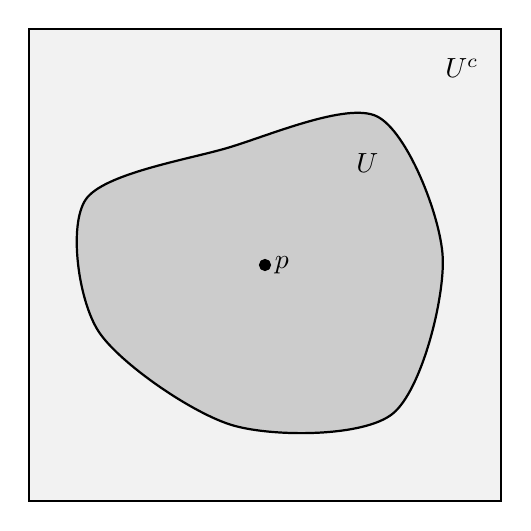
\begin{tikzpicture}
            \pgfmathsetseed{3}
            \draw[black, thick, fill=gray!10!white] (0,0) rectangle
            (6,6) node at (5.5, 5.5) {$U^c$};
            \draw[thick, fill=gray!40!white, xshift = 3cm, yshift=3cm,
            scale = 1.3] plot [smooth cycle, samples=7,domain={1:8}] 
            (\x*360/8+5*rnd:1cm+1cm*rnd) node at (1,1) {$U$};
            \filldraw[black] (3,3) circle (2pt) node[anchor=west] {$p$};
        \end{tikzpicture}   
        \hspace{2cm}
        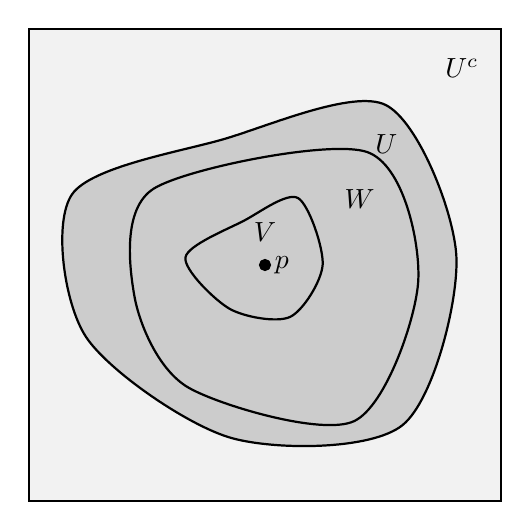
\begin{tikzpicture}
            \pgfmathsetseed{3}
            \draw[black, thick, fill=gray!10!white] (0,0) rectangle
            (6,6) node at (5.5, 5.5) {$U^c$};
            
            \draw[thick, fill=gray!40!white, xshift = 3cm, yshift=3cm,
            scale = 1.4] plot [smooth cycle, samples=7,domain={1:8}] 
            (\x*360/8+5*rnd:1cm+1cm*rnd) node at (1.1,1.1) {$U$};

            \draw[thick, fill=gray!40!white, xshift = 3cm, yshift=3cm, scale=1.2] plot [smooth cycle, samples=6,domain={3:9}] 
            (\x*360/8+5*rnd:1cm+1cm*rnd) node at (1,0.7) {$W$};
            
            \draw[thick, fill=gray!40!white, xshift = 3cm, yshift=3cm, scale=0.6] plot [smooth cycle, samples=6,domain={1:8}] 
            (\x*360/8+5*rnd:1cm+1cm*rnd) node at (0,0.7) {$V$};
            
            \filldraw[black] (3,3) circle (2pt) node[anchor=west] {$p$};
        \end{tikzpicture}     
    \end{center}
    \caption*{The first picture shows an arbitrary open set $U$
    containing $p$. In the second picture, we see that $U^c
    \subset W$, so the boundary of $W$ lives inside $U$. $V$ is disjoint from
    $W$, but contains $p$, so it also lives inside $U$.}
\end{figure*}


\end{proof}

\begin{problem}[Theorem 5.9] A topological space $X$ is normal if and
    only if for each closed set $A$ in $X$ and open set $U$ containing
    $A$ there exists an open set $V$ such that $A \subset A$ and
    $\overline{V} \subset U$.
\end{problem}

\begin{proof}
    Suppose that $X$ is normal. Let $A$ be a closed set, and 
    $U$ an open set about $A$. 
    Since $U^c$ is closed and disjoint from $A$, 
    there must exist a pair of disjoint open sets $V, W$ 
    such that $U^c \subset V$ and $A \subset W$.
    Next observe that since $V$ and $W$ are disjoint, we know
    that $W \subset V^c$. Since $V^c$ is closed, we also know that 
    $\overline{W} \subset V^c$. But $V^c \subset U$; Thus we have that 
    $A \subset W \subset \overline{W} \subset V^c \subset U$. Thus for 
    every closed $A$ and $U$ containing $A$, there exists an open 
    set $W$ such that $A \subset \overline{W} \subset U$, as desired.
    \\
    \\
    Now suppose that for a closed set $A$ and an open set $U$ containing 
    $A$ there exists an open set $V$ such that $A \subset V$ and $\overline{V} 
    \subset U$. Let $B$ be a closed set which is disjoint from $A$. Since 
    $A$ and $B$ have no limit points in common, we can see that for each $a \in A$, 
    there exists an open set $U_a$ such that $U_a \cap B = \emptyset.$ Thus 
    let $U' = \bigcup\limits_{a \in A} U_a$, which is an open set. 
    Then $U' \cap B = \emptyset$ by construction, and by assumption there 
    must exist an open set $W$ such that $A \subset W$ and $\overline{W} \subset
    U'$.
    Next observe that $\overline{U}^c$ is an open set which contains $B$, so by 
    assumption there exists a $W'$ such that $B \subset W' \subset \overline{W'}
    \subset \overline{U}^c$. Thus we see that $A \subset W$ and $B \subset W'$,
    and $W \cap W' = \emptyset$ since $W \subset U$ but $W' \subset \overline{U}^c$
    Since $A$ and $B$ were arbitrary closed sets, and can be contained in
    disjoint open sets,
    we have that the space is normal, which proves the assertion.
   
\end{proof}
\textbf{Presented in class 2/20}\\
\begin{problem}[Theorem 5.10] A topological space $X$ is normal if and
    only if for each pair of disjoint closed sets $A$ and $B$ there
    are disjoint open sets $U$ and $V$ such that $A \subset U$, $B
    \subset V$ and $\overline{U}\cap\overline{V} = \emptyset$.
\end{problem}

\begin{proof}
    First we prove the forward direction. Suppose that $X$ is a normal
    space. Then for every pair of disjoint closed sets $A$ and $B$ in
    $X$, there exist disjoint open sets such that $A \subset U$ and $B
    \subset V$. However, by Theorem 5.9, we know that there must exist
    open sets $U'$ and $V'$ such that $A \subset U' \subset
    \overline{U'} \subset U$ and $B \subset V' \subset \overline{V'}
    \subset U$. Since $U'$ and $V'$ are disjoint, this proves the
    existence of disjoint open sets containing $A$ and $B$ whose
    intersection of their closures is empty. \\
    \\
    Next, suppose that for every pair of disjoint closed sets $A$ and
    $B$, there are disjoint open sets $U$ and $V$ such that $A \subset
    U$ and $B \subset V$ and $\overline{U} \cap \overline{V} =
    \emptyset$. Since $A, B$ are arbitrary disjoint closed sets, $A
    \subset U$ and $B \subset V$ and $U \cap V = \emptyset$, $X$
    satisfies the conditions of a normal space, so $X$ must be normal.
    
\end{proof}

\begin{problem}[Theorem 5.11](The Incredible Shrinking Theorem.) A
    topological space $X$ is normal if and only if for each pair of
    open sets $U, V$ such that $U \cup V = X$, there exist open sets
    $U', V'$ such that $\overline{U'} \subset U$ and $\overline{V'}
    \subset V$ and $U' \cup V' = X$.
\end{problem}

\begin{proof}
    First we prove the forward direction. Suppose $X$ is normal
    and that $U, V$ are open sets such that $U \cup V = X$. Observe that
    $U^c \subset V$ and $V^c \subset U$. By Theorem 5.9
    there must exist open sets $U', V'$ such
    that 
    \vspace{-6mm}
    \begin{gather*}
    U^c \subset U' 
    \text{ , } \overline{U'} \subset V
     \text{, }\\ 
     V^c \subset V' \text{, } \overline{V'}
    \subset U.
    \end{gather*}
    Since $(V')^c$ is a closed and 
    $(V')^c \subset V$, we can apply Theorem 5.9 again to conclude that
    there must exist a set $U''$ such that 
    $$
    (V')^c \subset U'' \text{, } \overline{U''} \subset V.
    $$
    Now since $U''$ and $V'$ are open sets such that
    $\overline{U''} \subset V$, $\overline{V'} \subset U$, and $U''
    \cap V' \ne \emptyset$ because $(V')^c \subset U''$, we have that
    $U'' \cup V' = X$. 
    \begin{figure}[h!!]
        \centering
        \includegraphics[width = 0.9\textwidth]{sketch_them_5_11.jpg}
        % \caption{A visual aid for the forward direction of this proof,
        % where the set $U, V, V'$ and $U''$ are described in the
        % proof.}
    \end{figure}
    \newpage
    \noindent
Thus this finishes the proof in this direction.
Next we prove the other direction. Suppose that for every pair of
open sets $U, V \subset X$ such that $U \cup V = X$, there exists open
sets $U', V'$ such that $\overline{U'}\subset U$ and $\overline{V'}
\subset V$. 
\\
\\
Let $A$ and $B$ be disjoint closed sets in $X$. Observe that $A^c$,
$B^c$ are open sets such that $A^c \cup B^c = X$. Thus there must
exist open sets $U, V$ such that 
\[
  \overline{U} \subset A^c \text{ , } \overline{V} \subset B^c \text{, }
  U \cup V = X.  
\]
Next observe that 
\begin{gather*}
  (A^c)^c \subset (\overline{U})^c \subset U^c \implies A \subset (\overline{U})^c \subset U^c\\
  (B^c)^c \subset (\overline{V})^c \subset V^c \implies B \subset (\overline{V})^c \subset V^c 
\end{gather*}
Since $U \cup V = X$, we have that $U^c \cap V^c = \emptyset$ by
DeMorgan's laws. Hence, $(\overline{U})^c$ and $(\overline{V})^c$ are
disjoint open sets such that $A \subset (\overline{U})^c$ and 
$B \subset (\overline{V})^c$. Thus by definition, $X$ is normal.
\end{proof}

\noindent\rule{18cm}{1pt}
\noindent
\textbf{Exercise 5.12}\\
1. Describe an example of a topological space that is $T_1$ but not
$T_2$.\\
2. Describe an example of a topological space that is $T_2$ but not
$T_3$.\\
3. Describe an example of a topological space that is $T_3$ but not
$T_4$.\\
\noindent\rule{18cm}{1pt}
\begin{enumerate}
    \item Finite complement topology is an example. First, every set 
     of the form $X - \{p\}$ where $p \in X$ is open, so the
     complement $X - (X - \{p\}) = \{p\}$ is closed. Hence by 
     Theorem 5.1, $X$ is $T_1$. 
     \\
    Now suppose $X$ is $T_2$, Then for all $p, q \in X$ and $p \ne q$,
    there exists disjoint, open sets $U, V$ such that $p \in U$, $q
    \in V$. However, $U \cap V \implies V \subset U^c$. 
    But this is a contradiction since $U^c$ is finite, by
    construction, and $V$ must at least be infinite (since we know
    that $V^c$ is finite.) Thus $X$ is not $T_2$.
    \\
    \\
    Another example would be the countable complement topology, and
    the proof is almost exactly as the one presented for the finite
    complement topology.

    \item The harmonic set is $T_2$ but not $T_3$. This is because for
    any two points $p, q \in \mathbb{R}$ we can contain them in
    disjoint open sets $(a, b)$ and $(c, d)$ where $a < p < b < c < q
    < d$ or $c < q < d < a < p < b$. If either $p$ or $q$ are in $H$,
    then it is vacuously true that we can contain them in an open set
    disjoint from any open set containing another point because there
    are no open sets which contain elements of $H$.
    \\
    \\
    The harmonic set is not $T_3$ since (1) $H$ is a closed set (as it
    has no limit points) and (2) no open set can contain $H$.
    Therefore, it cannot be regular, and hence not $T_3$.
    
    \item In Exercise 5.4, we showed that $\mathbb{H}_\text{bub}$ is
    regular. Observe that by Exercise 4.10.3 every point on the
    $x$-axis can be contained in disjoint open sets, and it is trivial
    that two distinct points in $\{(x,y) : y > 0\}$ can be contained in
    disjoint open sets. Thus $\mathbb{H}_\text{bub}$ is $T_3$.
    However, by Exercise 4.10.5 the rationals and irrationals on the
    $x$-axis cannot be contained in disjoint open sets, and the
    rationals and irrationals are closed sets. Hence
    $\mathbb{H}_\text{bub}$ is not normal. Therefore,
    $\mathbb{H}_\text{bub}$ is $T_3$ but not $T_4$. 
    
\end{enumerate}
    
% \textbf{Exercise 5.13}\\
% \begin{tabular}{ |p{3cm}||p{3cm}|p{3cm}|p{3cm}|p{3cm}|  }
%     \hline
%     \multicolumn{5}{|c|}{Separation Properties of Topological Spaces}
%     \\
%     \hline
%     Topological Space& $T_1$ & Hausdorff & Regular & Normal\\
%     \hline
%     $\mathbb{R}_{\text{std}}$   & yes    &yes &yes &yes\\
%     \hline
%     $\mathbb{R}_{\text{std}}^n$ &yes  & yes   &yes &yes\\
%     \hline
%     Indiscrete &no & no&  no & yes\\
%     \hline
%     Discrete    &yes & yes&  yes &yes\\
%     \hline
%     Finite complement &   yes  & no &yes &yes\\
%     \hline
%     Countable complement & yes  & yes   &yes &yes \\
%     \hline
%     Lower limit ($\mathbb{R}_{\text{LL}}$) & yes  & yes &yes &yes\\
%     \hline
%     Double headed snake $\mathbb{R}_{+00}$ & yes & yes & yes & yes \\
%     \hline
%     $\mathbb{R}_{\text{har}}$ & yes & yes & yes & yes\\
%     \hline
%     $\mathbb{H}_{\text{bub}}$ & yes & yes & yes & yes\\ 
%     \hline
%     $\mathbb{Z}_{\text{arith}}$ & yes & yes & yes & yes\\
%     \hline
%     Lexicographically ordered square & yes & yes & yes & yes\\
%     \hline
%     $2^X$ & yes & yes & yes & yes\\
%     \hline
%    \end{tabular}
% \\
% \\
\noindent\rule{18cm}{1pt}
\noindent
\textbf{Exercise 5.14}
Show that $\mathbb{H}_{\text{bub}}$ is not normal. \\
\noindent\rule{18cm}{1pt}
\\
In the previous chapter, we saw that there does not exist disjoint
open sets $U$ and $V$ in $\mathbb{H}_{\text{bub}}$ such that
$\mathbb{Q} \in U$ and $\mathbb{R} - \mathbb{Q} \subset V$. However,
observe that $\mathbb{Q}$ and $\mathbb{R} - \mathbb{Q}$ are closed
sets. With this example we see that $\mathbb{H}_{\text{bub}}$ cannot
be a normal set. \\
\\
\begin{problem}[Theorem 5.15] Order topologies are $T_1$, Hausdorff,
regular and normal.
\end{problem}

\begin{proof}
    ($\mathbf{T_1.}$) Suppose $X$ has the order topology. 
    Let $a \in X$. Observe that $\{x \in X | a < x\} \cup \{x \in X \
    x > a\}$ is the union of two open sets, so it is open, and hence
    its complement, which is $\{a\}$, is closed. Thus every singleton
    set is a closed set, so $X$ is $T_1$.
    \\
    \\  
    (\textbf{Hausdorff.}) Consider two distinct
    points $a, b \in X$, and suppose without loss of generatlity that
    $a < b$. If there exists an element $c \in X$ such that $a < c < b$ then 
    \[
      \{x \in X | x < c\} \text{ and } \{x \in X | c < x\}  
    \]
    are two disjoint open sets which contain $a, b$ respectively.\\
    If there is no $c \in X$ such that $a < c < b$, then 
    \[
      \{x \in X | x < b\} \text{ and } \{x \in X | a < x\}  
    \]
    are two disjoint open sets which contain $a, b$ respectively.
    Thus $X$ is also a Hausdorff space.
    \\
    \\
    (\textbf{Regular.}) Now let $A$ be a closed set and suppose $x \notin A$. Since $x$ is
    not a limit point of $A$, we see that there must exist an open set
    $U$ which contains $x$ and $U \cap A = \emptyset$. Then a open set
    which is disjoint from $U$ and contains $A$ is $A^c - U$, which
    shows that the space is regular. 
\end{proof}

\begin{problem}[Theorem 5.16] Let $X$ and $Y$ be Hausdorff. Then $X
    \times Y$ is Hausdorff.
\end{problem}

\begin{proof}
    If $X$ and $Y$ are both Hausdorff, then for two distinct $p =
    (p_x, p_y)$ and $q = (q_x, q_y)$ both in $X \times Y$, there
    exists disjoint open sets $U_{p_x}, U_{q_x} \in \mathscr{T}_X$
    such that $p_x \in U_{p_x}$, $q_x \in U_{q_x}$ and another pair of
    disjoint sets $V_{p_y}, V_{q_y} \in \mathscr{T}_Y$ such that $p_y
    \in U_{p_y}$ and $q_y \in U_{q_y}$. Now observe that $p \in
    U_{p_x} \times U_{p_y}$ and $q \in V_{q_x} \times V_{q_y}$ while
    $U_{p_x} \times U_{p_y}$ is disjoint with $V_{q_x} \times
    V_{q_y}$. Since $p, q$ were arbitrary distinct points in $X \times
    Y$, we have that $X \times Y$ is a Hausdorff space. 
\end{proof}

\begin{problem}[Theorem 5.17] Let $X$ and $Y$ be regular. Then $X
    \times Y$ is regular.
\end{problem}

\begin{proof}
    Suppose $X$ and $Y$ are regular, and let $p = (p_x, p_y) \in X
    \times Y$. Suppose $p$ is contained in an open set $W$.
    Then there exists a basic open set of the form $U \times V$ which
    contains $p$ and where $U \in \mathscr{T}_X$ and $V \in
    \mathscr{T}_Y$. Now since $X$ and $Y$ are regular, we can use
    Theorem 5.8 to conclude the existence of open sets $U'$ and $V'$
    such that $p_x \in U'$ and $\overline{U'} \subset U$ and $p_y \in
    V'$ while $\overline{V'} \subset V$. Therefore, $\overline{U'}
    \times \overline{V'} \subset U \times V$.
    
    Now observe $p \in U' \times
    V'$ and that, by Exercise 4.34, $\overline{U'
    \times V'} = \overline{U'}\times\overline{V'} \subset U \times V$
    and hence is entirely
    contained in $W$. Since $p$ and $W$ were arbitrary, this shows
    that $X \times Y$ satisfies Theorem 5.8, allowing us to conclude
    that $X \times Y$ is a regular space. 
\end{proof}

\noindent
\textbf{Presented in class 2/25/19}\\
\begin{problem}[Theorem 5.19] Every Hausdorff is hereditarily
    Hausdorff. 
\end{problem}

\begin{proof}
    Let $Y$ be a subset of $X$, and consider the relative topology of
    $Y$ given by $$\mathscr{T}_Y = \{V | V = Y \cap U, U \in
    \mathscr{T}_X\}.$$ Since $X$ is Hausdorff, we know that for any
    distinct pair of points 
    $p, q \in Y$, which are obviously also points in $X$, there exist
    disjoint open sets $U', V' \in \mathscr{T}_X$ such that $p \in U'$
    and $q \in V'$. Next observe that $U'' = Y \cap U'$ and $V'' = Y
    \cap V'$ are two disjoint open sets in $\mathscr{T}_Y$ such that
    $p \in U''$ and $q \in V''$. Since $p, q$ were arbitrary points of
    $Y$, we have that $Y$ must also be a Hausdorff space. 
\end{proof}

\begin{problem}[Theorem 5.20] Every regular space is hereditarily
    regular.
\end{problem}
\begin{proof}
    Let $Y$ be a subset of $X$ endowed with the relative topology on
    $X$. Then consider $C$ closed in $(Y, \mathscr{T}_Y^{\text{
    rel}})$, and a point $x \in Y$ such that $x \notin C$. From
    Theorem 4.28, we know that $C$ is closed if and only if there
    exists a set $D$ closed in $(X, \mathscr{T}_X)$ such that $C = D
    \cap Y$. \\
    \\
    Since $X$ is regular, and we know that $x \notin D$, then for the
    set $D$ closed in $(X, \mathscr{T}_X)$ there exist disjoint sets
    $U, V \in (X, \mathscr{T}_X)$ such that $D \subset U$ and $x \in
    V$. Now observe that $U' = U \cap Y$ and $V' = V \cap Y$ are
    disjoint sets open in $\mathscr{T}_Y^{\text{ rel}}$ such that $C
    \subset U'$ and $x \in V'$. Since $C$ was an arbitrary closed set
    in $(Y, \mathscr{T}_Y^{\text{ rel}})$ and $x$ was a arbitrary
    point of $Y$ but not of $C$, the topological space $(Y,
    \mathscr{T}_Y^{\text{ rel}})$ satisfies the properties of being
    regular so $Y$ is a regular space.
\end{proof}
    
\begin{problem}[Theorem 5.23] Let $A$ be a closed subset of a normal
    space $X$. Then $A$ is normal when given the relative topology.
\end{problem}

\begin{proof}
    Let $X$ be a normal space, and consider the relative topology on
    $A$:
    $$
    \mathscr{T}_A^\text{ rel} = \{U | U = A \cap V \text{ where } V \in \mathscr{T}_X\}
    $$
    Now consider a pair of disjoint closed sets $D$, $C$ closed in
    $(A, \mathscr{T}_A^\text{ rel})$.
    \begin{figure}[h!]
        \centering
        \includegraphics[width = 0.5\textwidth]{figures_theorems_sect_5/sketch_thm_5_23.jpg}
        \caption{In this figure, we drew a closed set $C$ completely
        contained in $A$ and a closed set $D$ which shares limit
        points with $A$ in $(X, \mathscr{T}_X)$.}
    \end{figure}
    Then by Theorem 4.28, we know that there must exist sets $D'$ and
    $C'$ closed in $(X, \mathscr{T})$ such that $C = A \cap C'$ and $D
    = A \cap D'$. Now observe that since $C$ and $D$ are result of
    intersecting two sets which are closed in $(X, \mathscr{T}_X)$, we
    must have that $C$ and $D$ are also sets closed in $(X,
    \mathscr{T}_X)$. \\
    \\
    Now since $X$ is normal and $C$ and $D$ are disjoint and closed in
    $(X, \mathscr{T}_X)$, there must exist
    disjoint, open sets $U$ and $V$ in $(X, \mathscr{T}_X)$ such that $C
    \subset U$ and $D \subset V$. Next, let $U' = A \cap U$ and $V' =
    A \cap V$ and observe that (1) $U'$ and $V'$ are disjoint open
    sets in $(A, \mathscr{T}_A^\text{ rel})$ and (2) $C \subset U'$ and $D \subset
    V'$. This is because $C \subset A$, so if $C \subset U$ then we
    are certain that $C \subset U \cap A = U'$; an identical argument
    applies to $D$. Now since $C$ and $D$ were arbitrary
    closed sets of $A$, we have that $A$ is a normal space when given
    the relative topology. 
\end{proof}

\begin{exercise}[Exercise 5.25]
Let $Y$ be a subspace of a topological space
$X$, and let $A$ and $B$ be two disjoint closed subsets of $Y$ in the
subspace topology. Show that both $\overline{A} \cap B = \emptyset$
and $A \cap \overline{B} = \emptyset$, where the closures are taken in
$X$. 
\end{exercise}

\begin{solution}
If $A$ and $B$ are two disjoint closed sets in the subspace topology,
then observe that no point of one set is a limit point of the other.
Thus for every point of $a \in A$, we can construct a set $U_a \in
\mathscr{T}_Y$ such that $U_a \cap B = \emptyset.$ Similarly, for
every point $b \in B$ we can construct a set $U_b \in \mathscr{T}_Y$
such that $U_b \cap A = \emptyset.$ \\
\\
Let $a$ be a limit point of $A$ in $(X, \mathscr{T})$, and consider an
open set $U \in \mathscr{T}_X$ containing $a$. Then let $U' = U \cap
Y$, and observe that $U' \cap B = \emptyset$ because $A$ and $B$ are
disjoint closed sets in $(Y, \mathscr{T_Y})$. Thus we see that $a$
cannot be a limit point of $B$, so that $\overline{A}\cap B =
\emptyset$, where the closure is taken in $X$. We can repeat the same
argument for $B$ since the argument is symmetric, and conclude that $A
\cap \overline{B} = \emptyset$ as well, giving the desired result. 
\end{solution}

\begin{problem}[Theorem 5.26]
    The space $X$ is a completely normal space if and only if $X$ is
    hereditarily normal. 
\end{problem}

\begin{proof}
    Suppose $X$ is completely normal. Let $Y$ be a subset and consider
    any two disjoint, closed sets $C$ and $D$ in the subspace topology
    
    \[
        \mathscr{T}_{Y} = \{U | U = V \cap Y : V \in \mathscr{T}_X\}.
    \]
    By Exercise 5.25, these sets are separated in $X$.

    Since $C$ and $D$ are separated in $X$, there exist two disjoint
    open sets $A$, $B$ such that $C \subset A$, $D \subset B$.
    Therefore, $A \cap Y$ and $B \cap Y$ are two open sets in
    $\mathscr{T}_Y$ such that $C \subset A \cap Y$ and $B \cap Y$,
    which shows that $Y$ is normal. Since $Y$ was an arbitrary subset
    we have that $X$ is hereditarily normal.

    Suppose now that $X$ is heredetiarily normal, and consider two
    separated subsets $A$ and $B$ of $X$. Denote the subspace $A \cup
    B$ as $Y$. Then observe that 
    \[ 
        Y \cap \overline{B} = (A \cup B) \cap \overline{B} 
        = (A \cap \overline{B}) \cup (B \cap \overline{B}) = B.
    \]
    Thus $B$ is closed in $Y$, since
    $\overline{B}$ is closed in $X$, and by Theorem 4.28 this implies
    that $Y \cap \overline{B} = B$ is a closed set in the subspace
    $Y$. By analogous reasoning, we also have that $A$ is closed in
    $Y$.

    Since $X$ is heredetiarily normal, $Y$ is a subspace, and 
    $A, B$ are disjoint closed sets in $Y$, we can contain $A$ and $B$
    in disjoint open sets $U$ and $V$ in $Y$. However, we also know
    $U = U' cap Y$ and $V = V' \cap Y$ for $U', V' 
    \in \mathscr{T}_X$.
\end{proof}


\begin{problem}[Theorem 5.29] (The Normality Lemma). Let $A$ and $B$
    be subsets of a topological space $X$ and let $\{U_i\}_{i \in
    \mathbb{N}}$ and $\{V_i\}_{i \in \mathbb{N}}$ be two collections
    of open sets such that
    \begin{enumerate}
        \item $A \subset \bigcup\limits_{i \in \mathbb{N}} U_i$
        \item $B \subset \bigcup\limits_{i \in \mathbb{N}} V_i$\
        \item for each $i$ in $\mathbb{N}$, $\overline{U_i} \cap B =
        \emptyset$ and $\overline{V_i} \cap A = \emptyset$.
    \end{enumerate}
    Then there exist open sets $U$ and $V$ such that $A \subset U$, $B
    \subset V$, and $U \cap V = \emptyset$.
\end{problem}

\begin{proof}
    Suppose that (1) and (2) hold, and let 
    $$U =  \bigcup\limits_{n \in \mathbb{N}} A_n
    = \bigcup\limits_{n \in \mathbb{N}}
    \left(U_n - \bigcup\limits_{i = 1}^n \overline{V_i}\right)$$ 
    and 
    $$V = \bigcup\limits_{n \in \mathbb{N}} B_n 
    = \bigcup\limits_{n \in \mathbb{N}}
    \left(V_n - \bigcup\limits_{i = 1}^n \overline{U_i}\right).$$
    Note that $U$ and $V$ are open because they each
    are the countable union of open sets. This is because each
    $\bigcup\limits_{i = 1}^n\overline{U_i}$ and $\bigcup\limits_{i = 1}^n\overline{V_i}$ 
    finite unions of closed sets, and hence are closed.
    Thus each $U_n - \bigcup\limits_{i = 1}^n \overline{V_i}$ and 
    $V_n - \bigcup\limits_{i = 1}^n \overline{U_i}$ 
    are open sets by Theorem 3.15. 
    \\
    \\
    Now observe that $A \subset U$, $B \subset V$. We'll show this is
    true for $A$, since the argument that this is true for $B$ will be
    identical. Thus let $a \in A$. Then $a \in U_n$ for some $n \in
    \mathbb{N}$. However, $a \notin V_i$ for any $i \in \mathbb{N}$,
    so that $a \in U_n - \bigcup\limits_{i = 1}^n \overline{V_i}$.
    Therefore, $a \in \bigcup\limits_{n \in \mathbb{N}}
    \left(U_n - \bigcup\limits_{i = 1}^n \overline{V_i}\right) = U$,
    so that $A \subset U$.
    \\
    \\
    Finally, observe that $U \cap V = \emptyset$. If not, then there
    exists an $x \in U \cap V$. meaning that for some $m,n \in
    \mathbb{N}$, 
    \begin{align*}
        x \in U_n - \bigcup\limits_{i = 1}^n \overline{V_i}\\
        x \in V_m - \bigcup\limits_{i = 1}^m \overline{U_i}.
    \end{align*}
    Without loss of generality, suppose $n \le m$. Then by the second
    equation, we see that $x \notin U_i$ for $i \le m$. However, this
    implies that $x \notin U_n$ since $n \le m$, which contradicts the
    first above equation. Thus there cannot be such an $x$, and $U
    \cap V = \emptyset$.
\end{proof}
\textbf{Presented sketch 2/27/18}\\
\begin{problem}[Theorem 5.30] If $X$ is normal and $C = \cup_{i \in
    \mathbb{N}} K_i$ is the union of closed sets $K_i$ in $X$, then
    the subspace $C$ is normal. 
\end{problem}

\begin{proof}
    
\end{proof}

\begin{problem}[Theorem 5.31] Suppose a space $X$ is regular and
    countable. Then $X$ is normal.
\end{problem}

\begin{proof}
    Consider two sets $A$ and $B$. Since $X$ is regular, we know by an
    application of the definition that for all $a \in A$, there exist
    open sets $\{U_a\}$ such that $a \in U_a$ which are each disjoint
    with $\overline{B}$. Similarly, there must exist open sets
    $\{U_b\}$ such that $b \in U_b$ which are each disjoint with
    $\overline{A}$. \\
    \\
    Now by Theorem 5.8, we know that for each open set $U_a$
    containing $a$, there exists an open set $V_a$ such that $a \in
    V_a$ and $\overline{V_a} \subset U_a$. Similarly, for each open
    set $U_b$ containing $b$, there exists an open set $V_b$ such that
    $b \in V_b$ and $\overline{V_b} \subset U_b$ \\
    \\
    Observe that $A \subset \bigcup\limits_{a \in A}V_a$, $B \subset
    \bigcup\limits_{b \in
    B}V_b$, and that $\overline{V_b} \cap A = \overline{V_a} \cap B =
    \emptyset$ for all $a \in A$ and $b \in B$. Since $A, B$ are at
    most countable, the sets $\{U_a\}_{a \in A}$ and $\{U_b\}_{b \in
    B}$ are at most countable. 
    \\
    Thus by the Normality
    Lemma, we can then conclude there exist open sets $U$ and $V$ such
    that $A \subset U$ and $B \subset V$ while $U \cap V = \emptyset$.
    Therefore, we can conclude that $X$ is normal, which is what we
    set out to show.
\end{proof}

\noindent
\textbf{Presented 2/27/18}\\
\begin{problem}[Theorem 5.32] Suppose a space $X$ is regular and has a
    countable basis. Then $X$ is normal.
\end{problem}

\begin{proof}
    Consider two disjoint subsets $A$ and $B$ of $X$. Since they are
    disjoint, we know that for each $a \in A$, there exists an open
    set $U_a$ such that $U_a \cap B = \emptyset$ for all $a \in A$.
    Similarly for each $b \in B$, we know that there exists an open
    set $U_b \cap A = \emptyset$ for all $b \in B$. \\
    \\
    Observe that the sets $\{U_a\}$ and $\{U_b\}$ may or may not be
    countable. However, since we have a countable basis $\mathscr{B} =
    \{B_1, B_2, \dots\}$, we know by Theorem 4.1 that each $a \in A$
    is contained in some basis element $B_i$ such that $a \in B_i
    \subset U_a$, where $i \in \mathbb{N}$. Thus let $\mathscr{B}_A$
    be the set of basis elements such that $A \subset \bigcup_{B_A \in
    \mathscr{B}_A} B_A$. Similarly, every $b \in B$ is contained in a
    basis element $B_j$ such that $b \in B_j \subset U_b$, where $j
    \in \mathbb{N}$. Now let $\mathscr{B}_B$ by the set of basis
    elements such that $B \subset \bigcup_{B_B \in \mathscr{B}_B}
    B_B$. \\
    \\
    Now by Theorem 5.8, for each $a \in A$, there exists an open set
    $V_{j(a)}$ such that $a \in V_{j(a)}$ and $\overline{V_j(a)} \subset B_{i(a)}$
    where $j(a) \in \mathbb{N}$ and $i(a) \in \mathbb{N}$ is the index
    which corresponds to the set in $\{B_1, B_2, \dots\}$ such that $a
    \in B_{i(a)}$. Similarly for $B$, we know that for each $b \in B$
    there exists an open set $W_{j(b)}$ such that $b \in W_{j(b)}$ where $j \in
    \mathbb{N}$ and $\overline{W_j(b)} \subset B_{i(b)}$ where $i(b)$ is
    defined analogously for how we defined $i(a)$. \\
    \\
    Finally, observe that $A \subset \bigcup_{j \in \mathbb{N}} V_j$,
    $B \subset \bigcup_{j \in \mathbb{N}} W_j$, and that $V_j \cap B =
    W_j \cap A=\emptyset$ for each $j \in \mathbb{N}$. Since these
    conditions satisfy that the normality lemma, we have that $X$ is
    normal, which is what we set out to show.
\end{proof}


\end{document}
